% !TeX root = ../main.tex

以固定训练集的 $N_0=83{,}984$ 个好样本和 $N_1=6{,}016$ 个坏样本计算编码。
对某变量的第 $k$ 档，记好、坏样本数为 $n_{0k}$、$n_{1k}$，总档数为 $K$，
其中缺失、低收入及 96/98 等已定义的特殊档均计入 $K$。
两类样本在各档的平滑分布为：
\begin{equation}
  g_k=\frac{n_{0k}+\alpha}{N_0+\alpha K},\qquad
  b_k=\frac{n_{1k}+\alpha}{N_1+\alpha K},\qquad \alpha=0.5.
  \label{eq:smoothed-distributions}
\end{equation}

WOE 统一采用好样本分布除以坏样本分布：

\begin{equation}
  \mathrm{WOE}_k=\ln\frac{g_k}{b_k}.
  \label{eq:woe}
\end{equation}

因此，正 WOE 表示该档相对更多地聚集好样本，负 WOE 表示相对更多地聚集坏样本。
逐档 IV 贡献及变量总 IV 定义为
\begin{equation}
  \mathrm{IV}_k=(g_k-b_k)\ln\frac{g_k}{b_k},\qquad
  \mathrm{IV}=\sum_{k=1}^{K}\mathrm{IV}_k.
  \label{eq:iv}
\end{equation}

本报告选择列出\texttt{DebtRatio}和\texttt{NumberOfTimes90DaysLate}的分箱结果,
详见表~\ref{tab:debt-woe}、表~\ref{tab:late90-woe}
；其余变量的全表保存在配套 CSV 中。
第~\ref{sec:binning}~节方案执行后，各变量档数与该节初始设计一致，本轮未再次合并。
全部普通档人数至少为 779，好、坏样本数分别至少为 287、106，均通过预定要求。
96/98 档共 161 人，作为未知编码的特殊状态独立保留。

\begin{table}[!htbp]
  \centering
  \caption{DebtRatio 的完整训练分箱表}
  \label{tab:debt-woe}
  \footnotesize
  \setlength{\tabcolsep}{2.2pt}
  \renewcommand{\arraystretch}{1.05}
  \begin{tabular}{lrrrrrrrr}
\toprule
档位 & 人数 & 好 & 坏 & 坏率 & $g_k$ & $b_k$ & WOE & IV 贡献 \\
\midrule
$0$ & 2,445 & 2,240 & 205 & 8.38\% & 0.02668 & 0.03414 & -0.2467 & 0.00184 \\
$(0,0.4]$ & 45,827 & 43,201 & 2,626 & 5.73\% & 0.51438 & 0.43633 & 0.1646 & 0.01284 \\
$(0.4,0.6]$ & 12,978 & 11,965 & 1,013 & 7.81\% & 0.14247 & 0.16837 & -0.1670 & 0.00433 \\
$(0.6,1]$ & 7,654 & 6,867 & 787 & 10.28\% & 0.08177 & 0.13082 & -0.4700 & 0.02306 \\
$(1,10]$ & 3,763 & 3,368 & 395 & 10.50\% & 0.04011 & 0.06570 & -0.4936 & 0.01263 \\
$(10,100]$ & 2,744 & 2,625 & 119 & 4.34\% & 0.03126 & 0.01985 & 0.4540 & 0.00518 \\
$(100,+\infty)$ & 14,589 & 13,718 & 871 & 5.97\% & 0.16334 & 0.14478 & 0.1206 & 0.00224 \\
\midrule
合计 & 90,000 & 83,984 & 6,016 & 6.68\% & 1 & 1 & --- & 0.06212 \\
\bottomrule
\end{tabular}

\end{table}

\begin{table}[!htbp]
  \centering
  \caption{NumberOfTimes90DaysLate 的完整训练分箱表}
  \label{tab:late90-woe}
  \footnotesize
  \setlength{\tabcolsep}{2.2pt}
  \renewcommand{\arraystretch}{1.05}
  \begin{tabular}{lrrrrrrrr}
\toprule
档位 & 人数 & 好 & 坏 & 坏率 & $g_k$ & $b_k$ & WOE & IV 贡献 \\
\midrule
$0$ & 84,989 & 81,057 & 3,932 & 4.63\% & 0.96513 & 0.65340 & 0.3901 & 0.12159 \\
$1$ & 3,159 & 2,094 & 1,065 & 33.71\% & 0.02494 & 0.17704 & -1.9599 & 0.29811 \\
$2$ & 912 & 476 & 436 & 47.81\% & 0.00567 & 0.07253 & -2.5481 & 0.17035 \\
$\geq 3$ & 779 & 287 & 492 & 63.16\% & 0.00342 & 0.08183 & -3.1741 & 0.24887 \\
96/98（特殊） & 161 & 70 & 91 & 56.52\% & 0.00084 & 0.01520 & -2.8965 & 0.04161 \\
\midrule
合计 & 90,000 & 83,984 & 6,016 & 6.68\% & 1 & 1 & --- & 0.88053 \\
\bottomrule
\end{tabular}

\end{table}

\paragraph{一档独立核算}
DebtRatio 的 $(1,10]$ 档有 3,368 个好样本、395 个坏样本，变量共 $K=7$ 档。
将人数直接代入式~\eqref{eq:smoothed-distributions}--\eqref{eq:iv}：
\begin{equation}
  \begin{aligned}
    g_k&=\frac{3{,}368+0.5}{83{,}984+0.5\times7}=0.0401072,\qquad
    b_k=\frac{395+0.5}{6{,}016+0.5\times7}=0.0657031,\\
    \mathrm{WOE}_k&=\ln\!\left(\frac{0.0401072}{0.0657031}\right)\approx-0.4936,\qquad
    \mathrm{IV}_k\approx0.01263.
  \end{aligned}
  \label{eq:woe-hand-check}
\end{equation}

该档占全部坏样本的比例高于其占全部好样本的比例，因而 WOE 为负；
其档内坏样本率 10.50\% 也高于训练集总体的 6.68\%。
图~\ref{fig:woe-debt-late90} 展示各档编码：严重逾期的普通档随次数增加而 WOE 下降，
DebtRatio 则保留前文解释的非单调关系，96/98 不参与普通次数的排序。

\begin{figure}[!htbp]
  \centering
  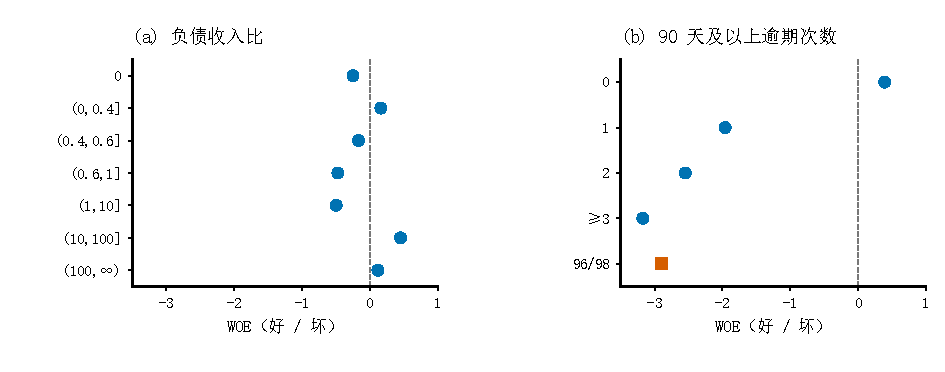
\includegraphics{figures/woe_debt_late90.pdf}
  \small
  \caption{DebtRatio 与历史严重逾期的 WOE 分布}
  \label{fig:woe-debt-late90}
  \begin{minipage}{\linewidth}
    \footnotesize
    注：点为训练集平滑 WOE，圆点为普通档，方块为 96/98 特殊档，虚线表示 WOE 为 0。
  \end{minipage}
\end{figure}

\paragraph{编码冻结与迁移}
保存切点、开闭端点、特殊路由和训练 WOE，验证客户按同一规则查表，
后续测试及新客户也使用该映射，不根据其标签重新计算编码。
若在训练集内部进行交叉验证，数据驱动的切点设计、预处理、WOE 和变量选择均须在各训练折内重做。
